Przedmiotem pracy jest stworzenie prototypowego serwera oraz klienta HTML5. Zadaniem serwera jest jest udostępnienie usługi uruchamiającej aplikacje oparte o biblioteki \emph{Qt} i KDE. Zdalny dostęp do aplikacji uruchomionej w środowisku serwera jest dostępny poprzez interfejs HTML5 udostępniany przez instancję serwera.

Użytkownik serwisu w celu skorzystania z aplikacji \emph{Qt} zainstalowanej na serwerze wchodzi na odpowiedni adres przy użyciu nowoczesnej przeglądarki internetowej. Następnie wybiera interesujący go program i przejmuje nad nim kontrolę. Jest w stanie wyświetlić program w przeglądarce, który wizualnie odpowiada rzeczywistej instancji uruchomionej na serwerze. Wszystkie akcje myszy oraz klawiatury przechwycone przez przeglądarke są wysyłane do serwera, dzięki czemu użytkownik ma pełną kontrolę nad uruchomioną aplikacją. Należy również zaimplementować odpowiednik menedżera okien (ang. window manager) po stronie klienta, aby udostępnić użytkownikowi funkcjonalność pracy z wieloma oknami --- przesuwanie, rozszerzanie, zamykanie, oraz opcjonalnie minimalizowanie oraz maksymalizowanie.

// TODO: Wymagania (ogólne)
// TODO: Przypadki użycia
// TODO: Zachowanie systemu / software'u
// TODO: Struktura systemu / software'u

Postawione zadanie w głównej mierze polega na rozwiązaniu czterech podstawowych problemów:
\begin{enumerate}
  \item komunikacja między klientem a serwerem,
  \item komunikacja między klientem a aplikacją,
  \item uzyskanie informacji o wyglądzie elementów graficznego interfejsu aplikacji,
  \item symulacja interakcji użytkownika z interfejsem aplikacji.
\end{enumerate}

Na rysunku \ref{fig:arch} przedstawiono ideowy schemat architektury systemu rozwiązującego powyższe kwestie. 
Podstawą projektu jest jego modułowość, która separuje logikę odpowiedzialną za udostępnianie interfejsu WWW inicjującego proces aplikacji Qt od części stanowiącej węzeł komunikacyjny pomiędzy klientem a aplikacją Qt działąjącą po stronie serwera.
Można również zauważyć bardzo wyraźne rozgraniczenie między dwoma kanałami przesyłu danych, które wynika z konieczności umożliwienia korzystania z serwera wielu klientom. 
Poniżej przedstawiono opis rozwiązań kolejnych problemów wraz z odniesieniem do odpowiednich części architektury na większym poziomie szczegółowości.

\begin{figure}
\centering
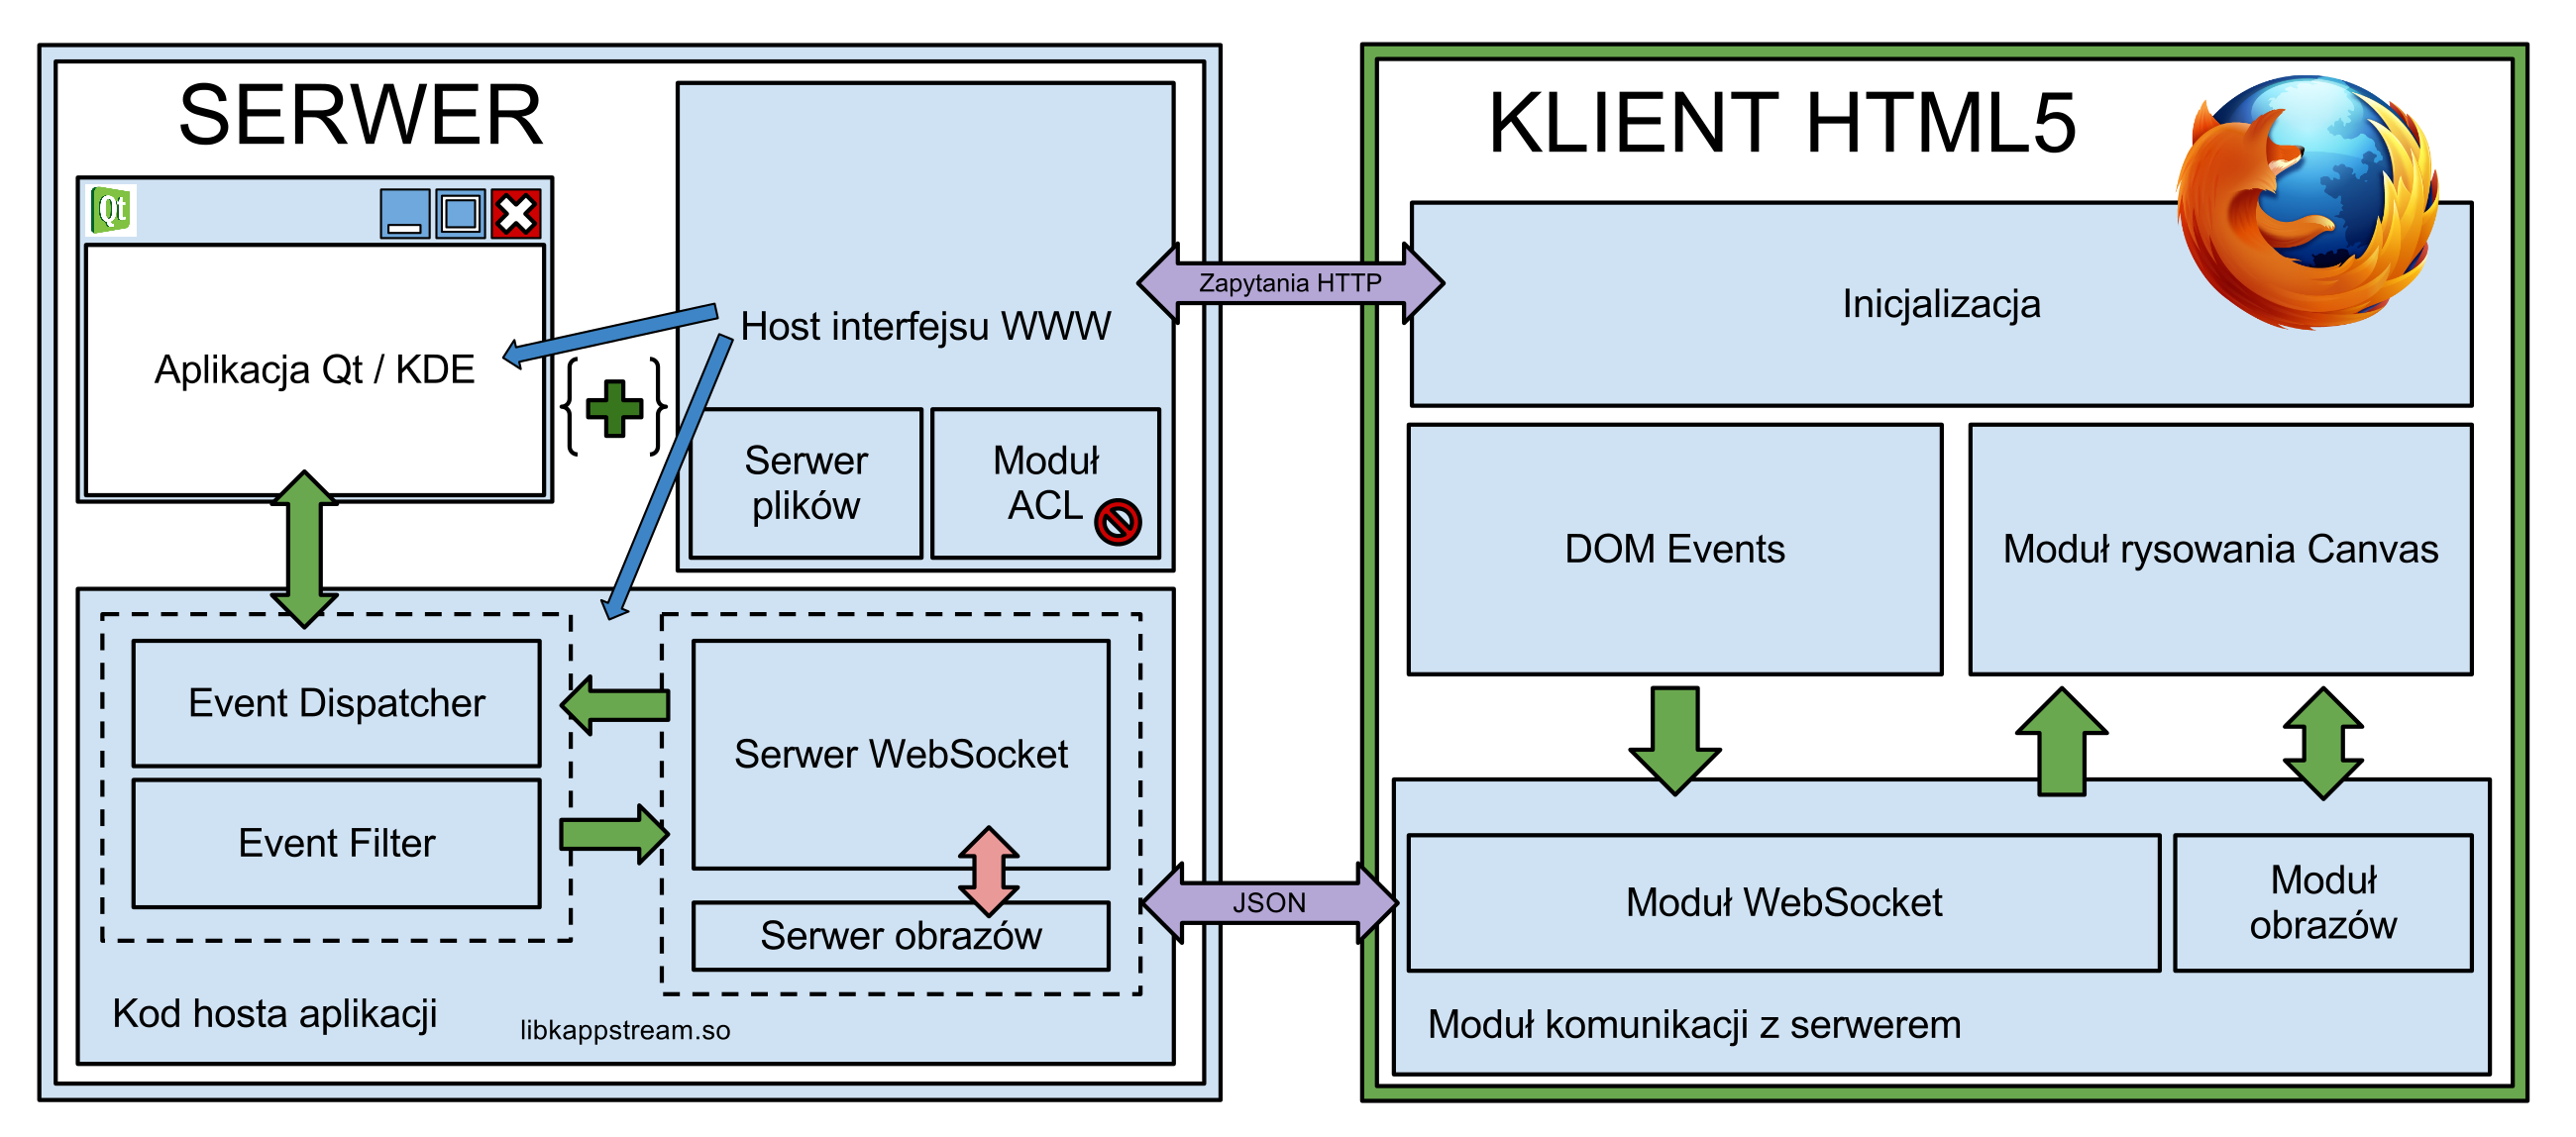
\includegraphics[width=1.0\linewidth]{img/arch}
\caption{Schemat architektury systemu.}
\label{fig:arch}
\end{figure}